\chapter{CP-Verletzung in B-Meson-Systemen}

\section{B-Mesonen und der Zerfallskanal \Decaychannel}
\subsection{Das Standardmodell der Teilchenphysik}
Im Standardmodell der Teilchenphysik gibt es 17 elementare Bausteine der Materie (siehe Abb. \ref{fig:standardmodell}): 12 Fermionen, davon 6 Quarks (u, d, c, s, t, b), die sich im engeren Sinne zur Materie hadronisieren oder Mesonen bilden, und 6 Leptonen (e, $\mathrm{\mu}$, $\mathrm{\tau}$ sowie die jweiligen Neutrinos $\mathrm{\nu_e}$, $\mathrm{\nu_{\mu}}$, $\mathrm{\nu_{\tau}}$). Von diesen 12 Fermionen existieren jeweils noch Antiteilchen (gleiche Eigenschaften, aber entgegengesetzte Masse). Das Standardmodell enthält weiterhin 4 Eichbosonen (Photon, Gluon, Z- und W$^{\pm}$-Boson), die die 3 der 4 elementaren Kräfte übertragen: die elektromagnetische, starke und schwache Wechselwirkung. Das für die Gravitation postulierte Graviton konnte bislang nicht nachgewiesen werden. Ergänzt wird das Standardmodell, durch das Higgs-Boson, welches als Teil des Higgs-Mechanismus den Elementarteilchen seine Masse verleiht und Gegenstand aktueller Forschung ist. Mit hoher Wahrscheinlichkeit gelang jüngst der Nachweis des Higgs am CERN \cite{higgs}.

\begin{figure}[hptb]
\centering
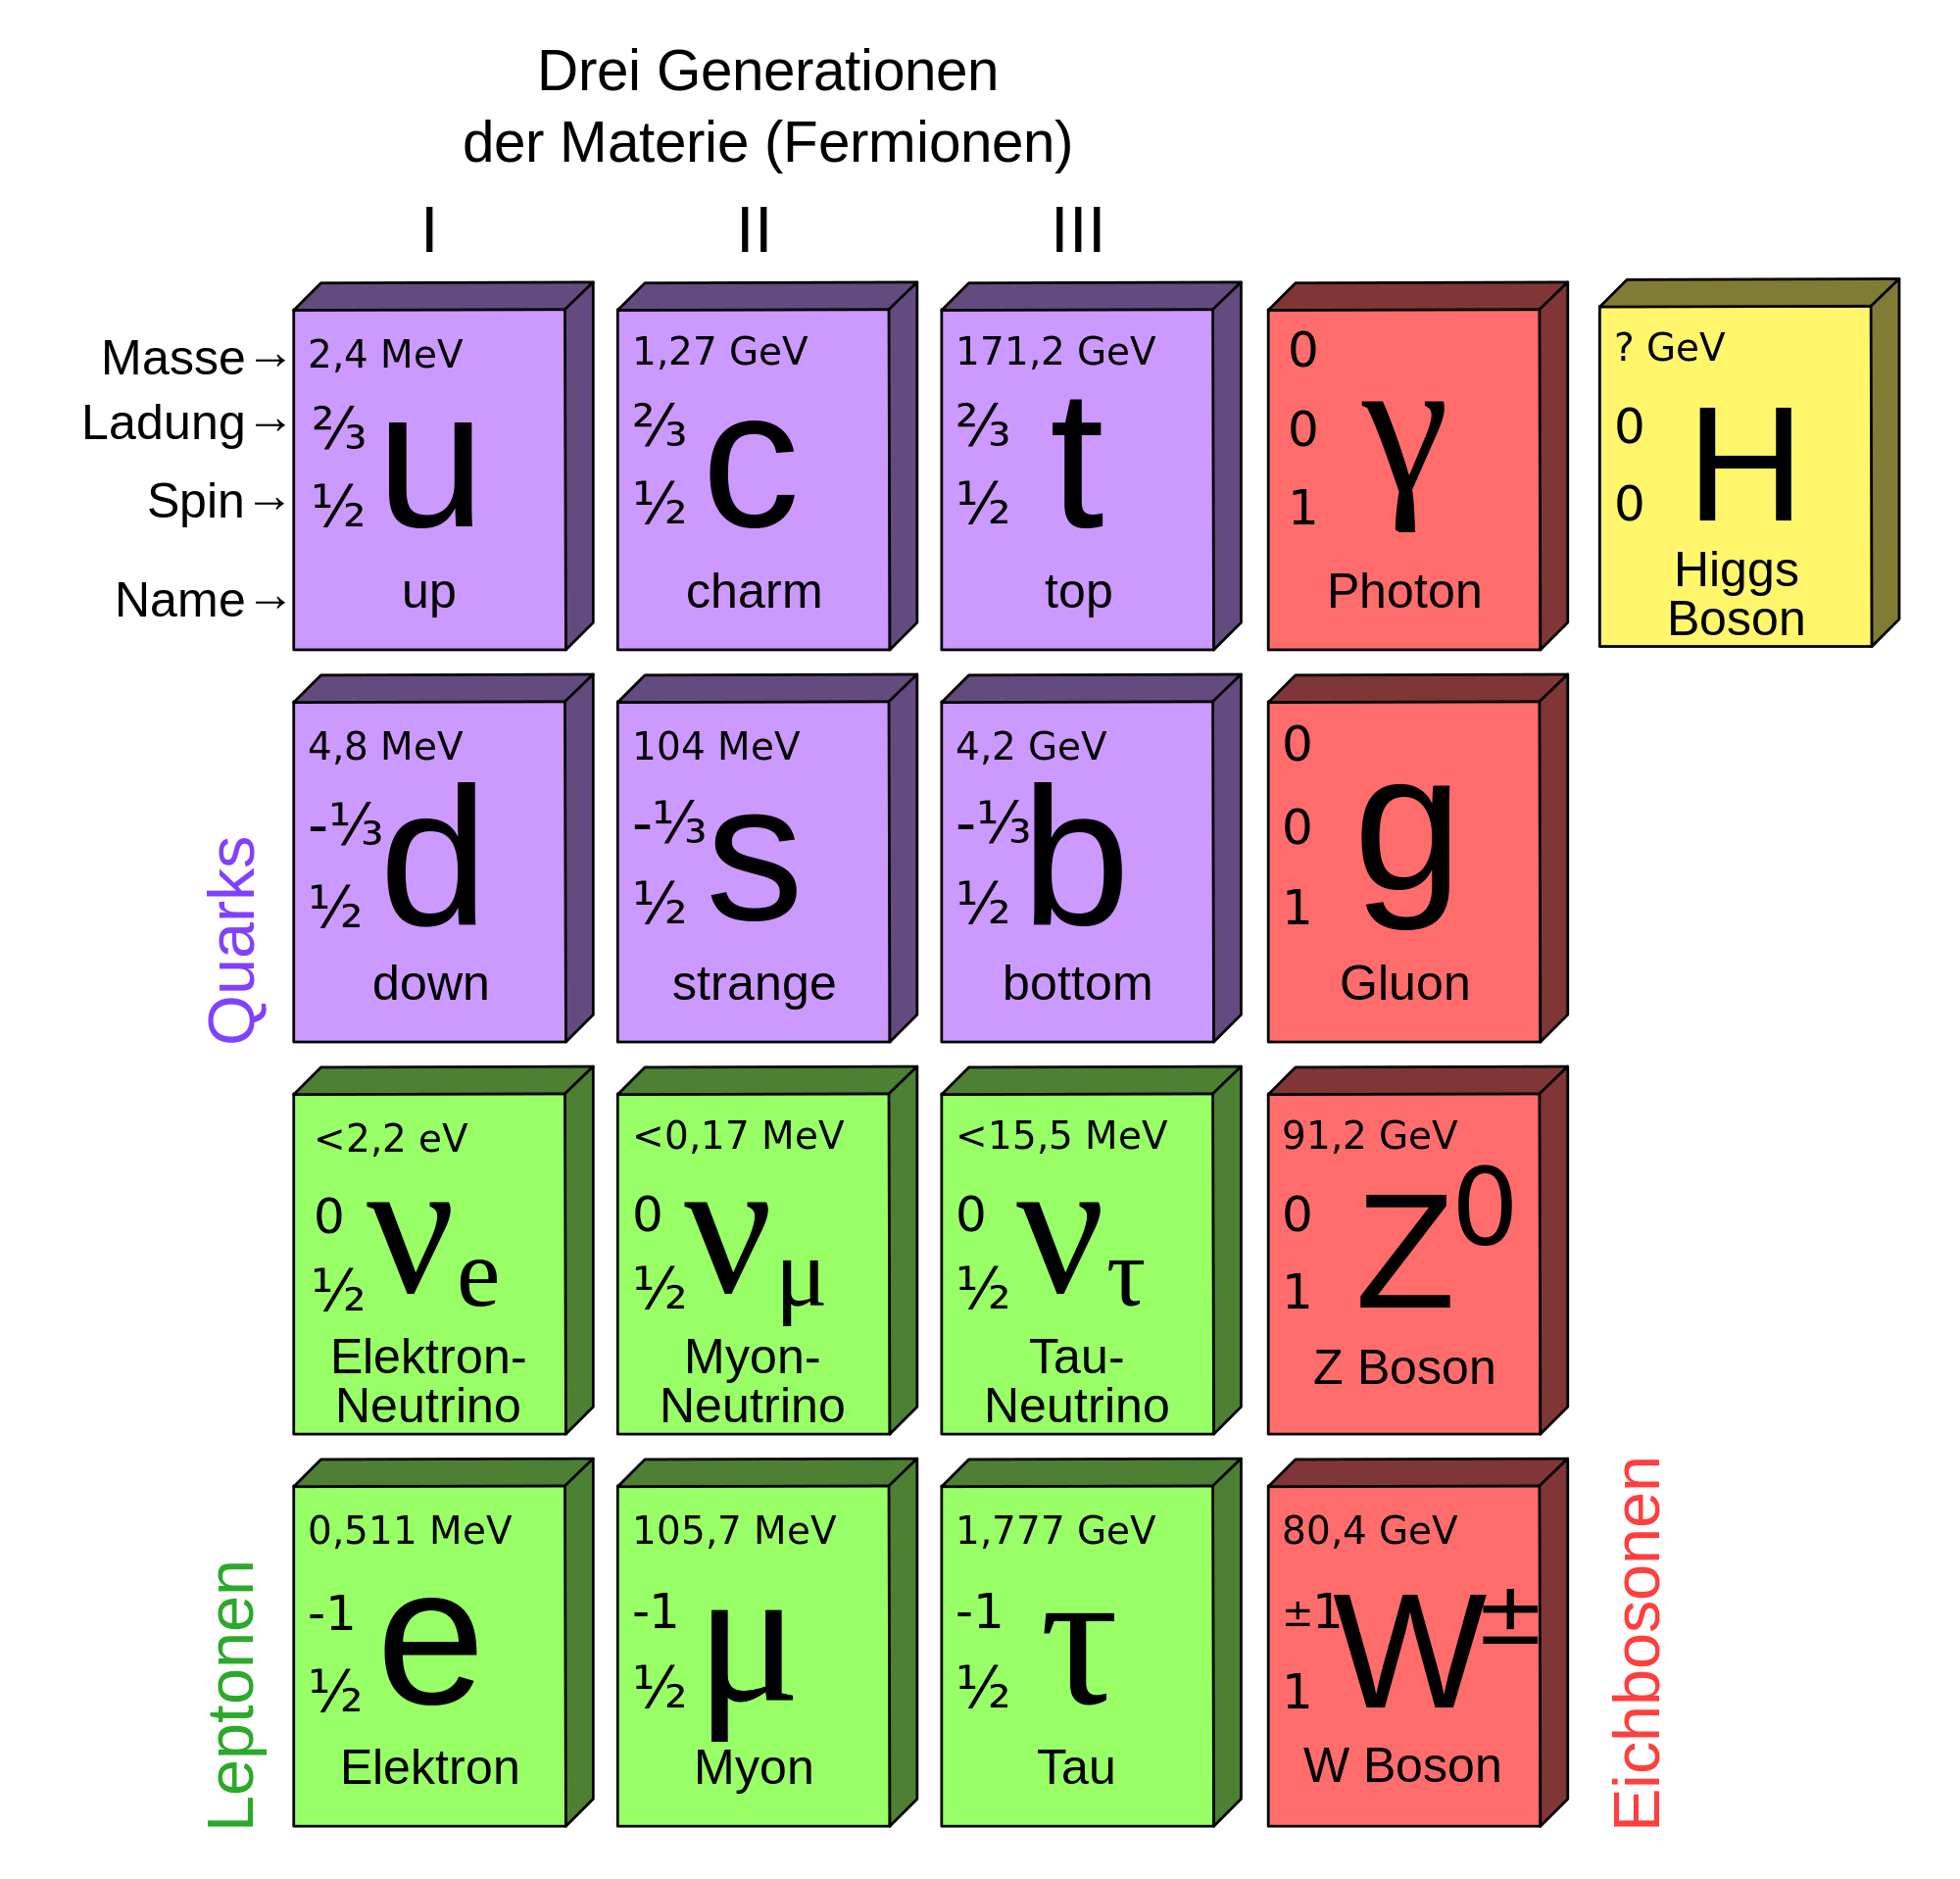
\includegraphics[width=0.5\textwidth]{standardmodell}
\caption{Das Standardmodell der Teilchenphysik \cite{wiki_standard}}
\label{fig:standardmodell}
\end{figure}

\subsection{B-Mesonen und ihre Mischung}
Mesonen sind Paare aus Quarks und Antiquarks beliebigen Flavours. B-Mesonen insbesondere bestehen aus einem Anti-b-Quark ($\mathrm{\overline{b}}$) mit einem u-, d-, c- oder s-Quark beziehungsweise aus der Kombination der jeweiligen Antiteilchen (Anti-B-Mesonen).

Die in dieser Arbeit betrachteten \Bd-Mesonen haben demnach die Quarkzusammensetzung $\Ket{\text{\Bd}} = \Ket{\overline{b}d}$ und sind elektrisch neutral. Solch neutrale Mesonen besitzen die Eigenschaft, dass sie sich in ihre Antiteilchen wandeln können und umgekehrt. Es findet folglich eine Oszillation zwischen \Bd\ und \Bdbar\ statt, die man auch Mischung nennt. Abbildung \ref{fig:bmixing} zeigt zwei mögliche Feynmangraphen für diesen Prozess. Innerhalb der Schleifen kann die Energieerhaltung kurzzeitig verletzt werden, sodass auch kurzerhand die deutlich schweren top-Quarks enstehen können. Zu diesem Mischungsprozess leisten sie sogar einen dominanten Beitrag. Präzise Messungen der \Bd-Mischung erlauben Aussagen bspw. über die top-Masse und grenzen damit das Standardmodell ein, gleichzeitig erhofft man sich, durch noch präzisere Messungen Hinweise auf \glqq neue Physik\grqq\ zu finden, die sich dann in kleinsten Korrekturen innerhalb der Schleife bemerkbar machen würden.

\begin{figure}[hptb]
\centering
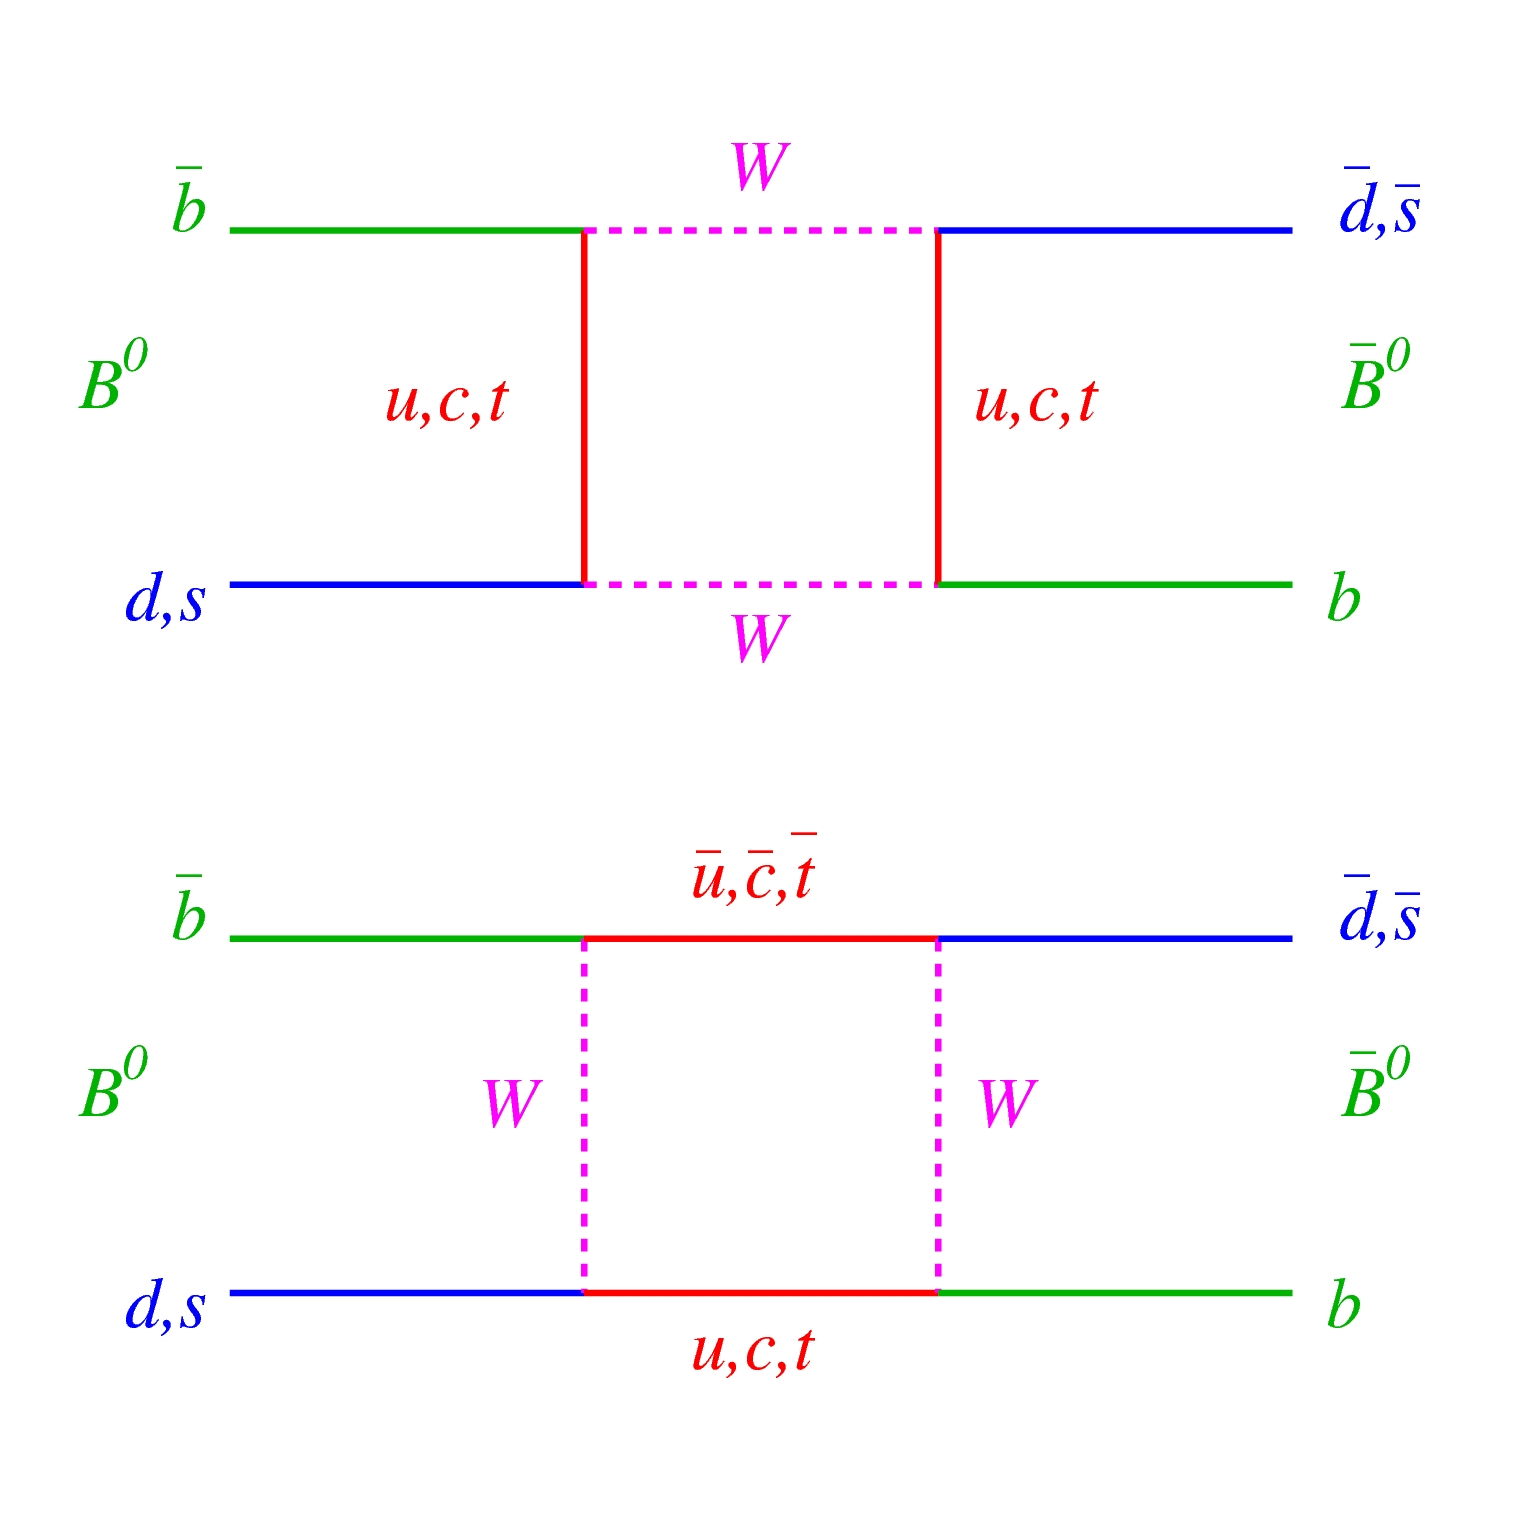
\includegraphics[width=0.5\textwidth]{bmixing}
\caption{Feynmangraphen zur Mischung von \Bd- und \Bdbar-Mesonen}
\label{fig:bmixing}
\end{figure}


\subsection{Der Zerfallskanal \Decaychannel}
In dieser Arbeit wird der Zerfallskanal \Decaychannel\ betrachtet. Abbildung \ref{fig:decay} zeigt entsprechende Feynmangraphen. Jener Kanal ist auch als \glqq goldener\grqq\ Zerfallskanal für die Messung der \CP-Verletzung bekannt. Hintergrund ist, dass der Endzustand $\Ket{\JPsi\Kshort}$ ein \CP-Eigenzustand ist ($\text{\CP}\Ket{\JPsi\Kshort} = - \Ket{\JPsi\Kshort}$). Damit können sowohl \Bd- als auch \Bdbar-Mesonen in den Endzustand zerfallen. Da \Bd\ und \Bdbar\ auch noch mischen, kommt es zu \CP-verletzenden Interferenzen der Zerfallsamplituden für den direkten Zerfall und den Zerfall nach vorheriger Miischung. Die Teilchen $\JPsi$ und $\Kshort$ haben die Flavoureigenzustände $\Ket{\JPsi} = \Ket{c\overline{c}}$ sowie $\Ket{\Kshort} = \tfrac{1}{\sqrt{2}}\left(\Ket{d\overline{s}}-\Ket{s\overline{d}}\right)$. Diese Teilchen sind ebenfalls nicht stabil und zerfallen unter anderem weiter gemäß $\JPsi \rightarrow \mu^+\mu^-$ und $\Kshort \rightarrow \pi^+\pi^-$, was zur Rekonstruktion der \Bd-Mesonen im Detektor genutzt wird.

\begin{figure}[hptb]
\centering
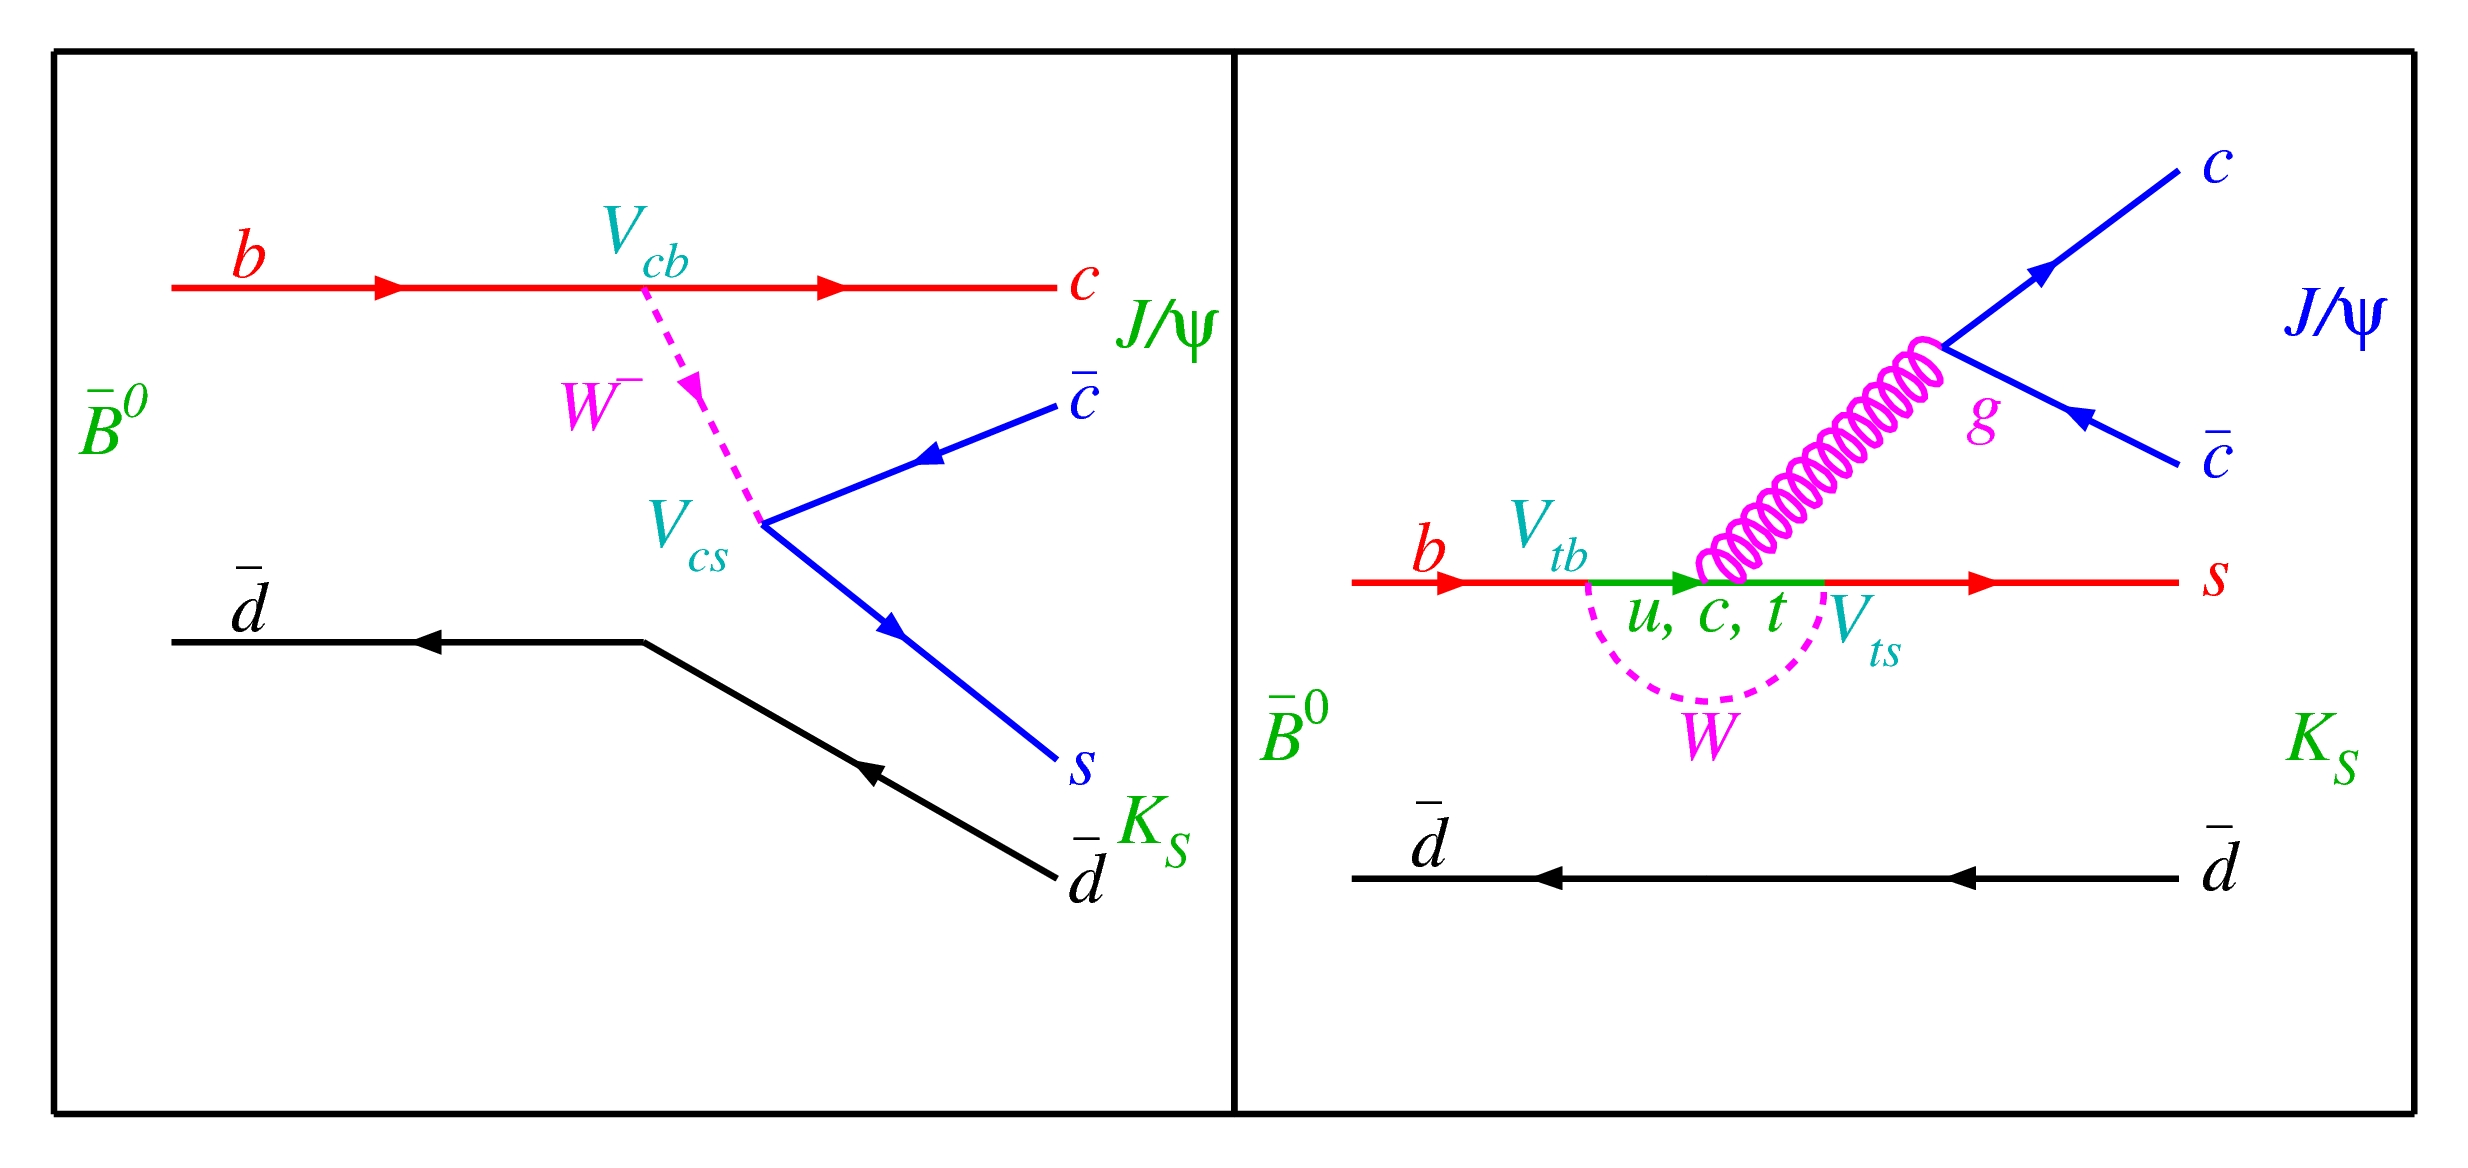
\includegraphics[width=\textwidth]{bd2jpsikshort}
\caption{Feynmangraph zum Zerfall \Decaychannel. Links: Baumdiagramm, rechts: Pinguindiagramm}
\label{fig:decay}
\end{figure}

\section{Diskrete Symmetrietransformationen}
Symmetrien sind in der Physik von zentraler Bedeutung. Gemäß dem Noether-Theorem existiert in der klassischen Physik zu jeder kontinuierlichen Symmetrie eine Erhaltungsgröße. In quantenmechanischen Systemen lassen sich drei diskrete Symmetrietransformationen betrachten:
\begin{enumerate}
\item \textbf{Parität $\mathcal{P}$:} \\
      Bei der Paritätsoperation wird das Vorzeichen der kartesischen Ortskoordinaten umgekehrt. Dies entspricht einer Punktspigelung.
\item \textbf{Ladungskonjugation $\mathcal{C}$:} \\
      Jedes Teilchen wird durch sein Antiteilchen ersetzt.
\item \textbf{Zeitumkehr $\mathcal{T}$:} \\
      Das Vorzeichen auf der Zeitachse wird umgekehrt. Da in der vorligenden Arbeit allerdings nur die CP-Verletzung gemessen werden soll, wird die Zeitumkehr im folgenden vernachlässigt.
\end{enumerate}
Entgegen der klassischen Intuition konnte Wu 1956 nachweisen, dass die Parität im $\beta$-Zerfall und damit in der schwachen Wechselwirkung nicht erhalten ist. Weitere Experimente zeigen, dass die schwache Wechselwirkung die Parität maximal verletzt: Neutrinos, die nur schwach wechselwirken können, sind stets \glqq linkshändig\grqq\ (Spin und Impuls antiparallel), Antineutrinos dagegen immer \glqq rechtshändig\grqq\ (Spin und Impuls parallel). Da der Spin im Gegensatz zum Impuls invariant unter $\mathcal{P}$-Transformation ist, würde diese Operation aus einem linkshändigen Neutrino ein rechtshändiges machen, was in der Natur nicht realisiert ist.

Damit ist offensichtlich, dass die schwache Wechselwirkung auch die Ladungskonjugation verletzt: Wendet man die $\mathcal{C}$-Transformation auf ein linkshändiges Neutrino an, so erhält man ein linkshändiges Antineutrino. Dieses existiert aber wie bereits erwähnt nicht. Analog gilt die Überlegung auch für Antineutrinos.

\subsubsection{Scheinbare $\mathcal{CP}$-Invarianz}
Wendet man nun aber die Transformationen $\mathcal{P}$ und $\mathcal{C}$ direkt hintereinander an, so ergibt sich zunächst kein Widerspruch zur Natur (siehe Abb. \ref{fig:cp_invarianz}). Aus einen linkshändigen Neutrino wird ein rechtshändiges Antineutrino. Im Jahre 1964 wurde dann allerdings im Zerfall neutraler K-Mesonen erstmals $\mathcal{CP}$-Verletzung nachgewiesen. \cite{kleinknecht}

\begin{figure}[hptb]
\centering
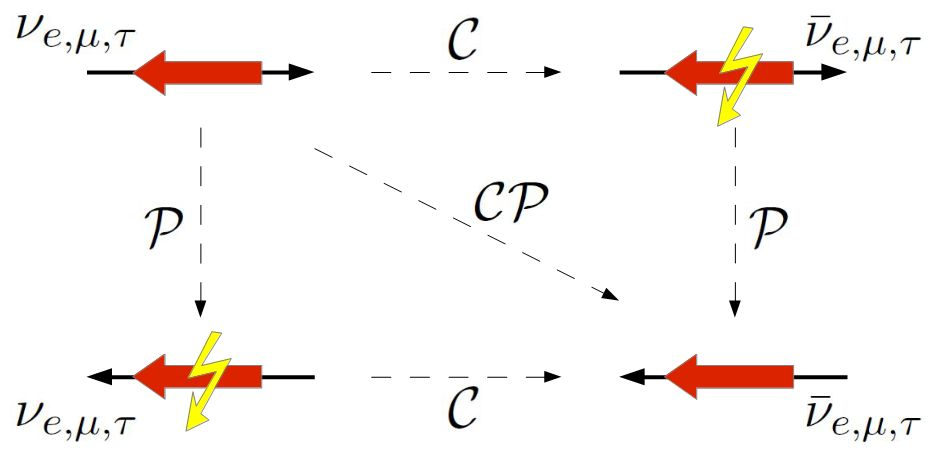
\includegraphics[width = 0.8\textwidth]{cp_invarianz}
\caption{Scheinbare $\mathcal{CP}$-Invarianz: Während eine reine $\mathcal{P}$- oder $\mathcal{C}$-Transformation zu in der Natur nicht realisierten Zuständen führt, scheint es bei der kombinierten $\mathcal{CP}$-Transformation keinen Widerspruch zu geben (dünne Pfeile: Impulsausrichtung, dicke Pfeile: Spinausrichtung).}
\label{fig:cp_invarianz}
\end{figure}

Diese Arbeit beschäftigt sich mit der \CP-Verletzung im B-Mesonen-System. Eine genaue Kenntnis der \CP-Verletzung ermöglicht Präzisionstests des Standardmodells. Weiterhin ist insbesondere das B-Meson-System sensitiv für \glqq neue Physik\grqq\, da durch Schleifen innerhalb der Prozesse (siehe Abb. \ref{fig:bmixing} und \ref{fig:decay}) Beiträge von Theorien jenseits des Standardmodells möglich sind und evtl. zu Abweichungen führen. Dabei unterscheidet man prinzipiell drei Arten von \CP-Verletzung:
\begin{enumerate}
\item \CP-Verletzung in der Mischung
\item direkte \CP-Verletzung
\item \CP-Verletzung in der Interferenz (indirekte \CP-Verletzung)
\end{enumerate}
Die nun folgenden Herleitungen und Erklärungen der drei Arten der \CP-Verletzung basieren auf den Ausführungen aus \cite{kleinknecht}.

\section{\CP-Verletzung in der Mischung}
Die Zeitentwicklung der Flavoureigenzustände zum Zeitpunkt t=0 $\Ket{\text{\Bd}} = \Ket{\overline{b}d}$ und $\Ket{\text{\Bdbar}} = \Ket{b\overline{d}}$, die sich unter \CP-Transformation gemäß
\begin{align}
\text{\CP}\Ket{\text{\Bd}} = -\Ket{\text{\Bdbar}} \qquad \text{\CP}\Ket{\text{\Bdbar}} = -\Ket{\text{\Bd}}
\end{align} 
verhalten, lässt sich phänomenologisch durch die Schrödinger-Gleichung
\begin{align}
\im \diff{}{t}\begin{pmatrix} \Ket{\text{\Bd}} \\ \Ket{\text{\Bdbar}} \end{pmatrix} = \left(M - \frac{\im}{2} \Gamma\right) \begin{pmatrix} \Ket{\text{\Bd}} \\ \Ket{\text{\Bdbar}} \end{pmatrix}
\end{align}
beschreiben. Der Hamiltonoperator $\mathcal{H}:=\left(M - \frac{\im}{2} \Gamma\right)$ setzt sich zusammen aus dem hermiteschen Massenoperator $M$ und dem ebenfalls hermiteschen Zerfallsoperator $\Gamma$. $\mathcal{H}$ selbt ist nicht hermitesch wegen des möglichen Zerfalls des Teilchens. Aus der $\mathcal{CPT}$-Erhaltung folgt $M_{11}=M_{22}=:M$ bzw. $\Gamma_{11}=\Gamma_{22}=:\Gamma$. Die nichtverschwindenden Elemente abseits der Diagonalen $M_{12}=M_{21}^*$, $\Gamma_{12}=\Gamma_{21}^*$ parametrisieren die \Bd-\Bdbar-Mischung. Offensichtlich entsprechen die Flavoureigenzustände nicht den Eigenzuständen von $\mathcal{H}$. Diagonalisieren von $\mathcal{H}$ liefert die Eigenzustände
\begin{align}
\Ket{B_h} &= p \Ket{\text{\Bd}} - q \Ket{\text{\Bdbar}} \label{eq:b_heavy}\\ 
\Ket{B_l} &= p \Ket{\text{\Bd}} + q \Ket{\text{\Bdbar}}, \qquad \text{mit} \quad |p|^2 + |q|^2 = 1, \label{eq:b_light}
\end{align}
mit definierten Massen $m_{h/l}$ und Zerfallsbreiten $\Gamma_{h/l}$ sowie den Eigenwerten  $m_{h/l}-\frac{\im}{2}\Gamma_{h/l}$. Dementsprechend gilt für die zeitliche Entwicklung der Zustände:
\begin{align}
\nonumber \Ket{B_{h/l}(t)} &= \e^{-\im m_{h/l}t-\frac{1}{2}\Gamma_{h/l}t}\Ket{B_{h/l}(0)} \\
                           &= \e^{-\gamma_{h/l}t}(p\Ket{\text{\Bd}} \mp q\Ket{\text{\Bdbar}}), \qquad
 \text{mit} \quad \gamma_{h/l} = \im m_{h/l}+\frac{\Gamma_{h/l}}{2}
\end{align}
Umgeschrieben auf die Flavoureigenbasis erhält man:
\begin{align}
\nonumber \Ket{\text{\Bd}(t)} &= \frac{1}{2p}\left(\Ket{B_h} + \Ket{B_l}\right) \\
                       &= \frac{1}{2}\left[ (\e^{-\gamma_h t}+\e^{-\gamma_l t})\Ket{\text{\Bd}} - \frac{q}{p}(\e^{-\gamma_h t}-\e^{-\gamma_l t})\Ket{\text{\Bdbar}}\right] \label{eg:b(t)}
\end{align}
Die Wahrscheinlichkeit für den Übergang eines $\Ket{\text{\Bd}}$ (zum Zeitpunkt $t=0$) in ein $\Ket{\text{\Bdbar}}$ beträgt:
\begin{align}
\nonumber P(\text{\Bd}\rightarrow\text{\Bdbar})(t) &= |\Braket{\text{\Bdbar}|\text{\Bd}(t)}|^2 \\
                                        &= \frac{1}{4} \left|\frac{q}{p}\right|^2 \left[\e^{-\Gamma_h t} + \e^{-\Gamma_l t} - 2\e^{-\frac{1}{2}(\Gamma_h + \Gamma_l) t}\cos(\Delta m_d t)\right]
\end{align}
Hierbei wird die Oszillationsdifferenz $\Delta m_d := m_h - m_l$ definiert, die aus der Massendifferenz der beiden Masseneigenzustände resultiert. Analog gilt für die Übergangswahrscheinlichkeit eines $\Ket{\text{\Bdbar}}$ in ein $\Ket{\text{\Bd}}$:
\begin{align}
P(\text{\Bdbar}\rightarrow \text{\Bd})(t) = \frac{1}{4} \left|\frac{p}{q}\right|^2 \left[\e^{-\Gamma_h t} + \e^{-\Gamma_l t} - 2\e^{-\frac{1}{2}(\Gamma_h + \Gamma_l) t}\cos(\Delta m_d t)\right] 
\end{align}
Folglich kommt es in der Mischung zur \CP-Verletzung, wenn die Oszillation ungleichmäßig verläuft, anders ausgedrückt:
\begin{align}
\text{\CP-Verletzung in der Mischung} \qquad \Longleftrightarrow \qquad \left|\frac{p}{q}\right| \neq 1 
\end{align}

\section{Direkte \CP-Verletzung}
Die Zerfallsamplituden der neutralen $\text{\Bd}$-Mesonen in einen Endzustand $\Ket{f}$ bzw. seinen \CP-konjugierten Zustand $\Ket{\overline{f}}$ sind definiert als
\begin{alignat}{2}
\nonumber A_f &= \Braket{f|\mathcal{H}|\text{\Bd}}, && \qquad A_{\overline{f}} = \Braket{\overline{f}|\mathcal{H}|\text{\Bd}}, \\
          \overline{A_f} &= \Braket{f|\mathcal{H}|\text{\Bdbar}}, && \qquad  \overline{A_{\overline{f}}} = \Braket{\overline{f}|\mathcal{H}|\text{\Bdbar}}. \label{eq:decay_amplitudes}
\end{alignat}
Ist \CP erhalten, dann sollten die Zerfallsraten, ergo auch die Zerfallsamplituden eines $\text{\Bd}$ nach $f$ sowie eines $\text{\Bdbar}$ nach $\overline{f}$ gleich sein. Dies bedeutet:
\begin{align}
\text{Direkte \CP-Verletzung} \qquad \Longleftrightarrow \qquad \frac{|A_f|}{|\overline{A_{\overline{f}}}|} \neq 1 \quad \text{bzw.} \quad \frac{|\overline{A_f}|}{|A_{\overline{f}}|} \neq 1
\end{align}


\section{\CP-Verletzung in der Interferenz}
Die Zustände \ref{eq:b_heavy} und \ref{eq:b_light} haben eine nahezu gleiche Anzahl an Zerfällskanäle. Dies hat zur Folge, dass die Lebensdauern des schweren und leichten Zustands innerhalb weniger Prozent gleich sind:
\begin{align}
\Gamma := \Gamma_h = \Gamma_l \label{eq:Gamma}
\end{align}
Weiterhin sagt das Standard Modell nur eine kleine \CP-Verletzung in der \Bd - \Bdbar - Mischung voraus, sodass
\begin{align}
\left|\frac{p}{q}\right| = 1 \qquad \text{in } \mathcal{O}(10^{-3}). \label{eg:pq_approx}
\end{align}
Für das B-Meson-System bleibt daher nur die Möglichkeit der \CP-Verletzung in der Interferenz der Amplituden von Zerfall nach Mischung und direktem Zerfall (siehe Abb. \ref{fig:interferenz}). 
\begin{figure}[hptb]
\centering
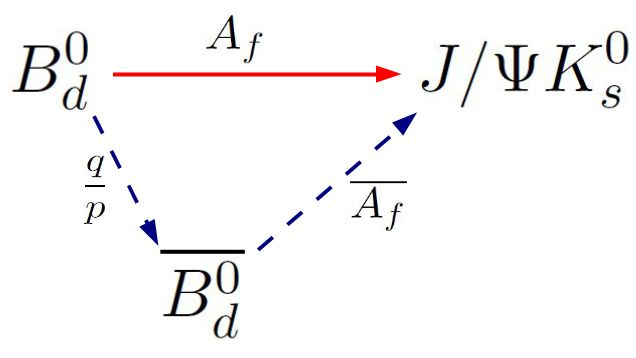
\includegraphics[width=0.5\textwidth]{interferenz}
\caption{Schema für die \CP-Verletzung in der Interferenz. Es interferieren die Amplituden für den direkten Zerfall (rot) mit der Amplitude für den Zerfall nach vorheriger Mischung (blau).}
\label{fig:interferenz}
\end{figure}
Der in dieser Arbeit betrachtete Zerfallskanal $B_d^0 \rightarrow J/\Psi K_s^0$ hat einen \CP-Eigenzustand als Endzustand (\CP $\Ket{\JPsi\Kshort} = -\Ket{\JPsi\Kshort}$). In Anlehnung an \ref{eq:decay_amplitudes} sind die Zerfallsamplituden hier definiert als
\begin{align}
\nonumber A_f := \Braket{f|\text{\Bd}(t)}, \qquad \overline{A_{f}} := \Braket{f|\text{\Bdbar}(t)}
\end{align}
Mit Blick auf die Zerfallsamplituden der Masseneigenzustände wird die komplexe Größe
\begin{align}
\lambda_f := \frac{q\overline{A_f}}{pA_f} \label{eq:lambda}
\end{align}
definiert. Ausgehend von Gleichung \ref{eg:b(t)} sowie mit Hilfe fer Gleichungen (\ref{eq:Gamma}), (\ref{eg:pq_approx}) und (\ref{eq:lambda}) gilt für die Zerfallsrate eines anfänglich reinen \Bd-Zustands:
\begin{align}
\nonumber \Gamma (\text{\Bd} \rightarrow \JPsi\Kshort) &= \frac{1}{4}\left| (\e^{-\gamma_h t}+\e^{-\gamma_l t})A_f - \frac{q}{p}(\e^{-\gamma_h t}-\e^{-\gamma_l t})\overline{A_f}\right|^2 \\
&= \frac{1}{2} \left|A_f\right|^2\e^{-\Gamma t} \left[1+|\lambda_f|^2 + (1-|\lambda_f|^2)\cos(\Delta m_d t) - 2\mathrm{Im}(\lambda_f)\sin(\Delta m_d t)\right] \label{eq:bd}
\end{align}
Analog:
\begin{align}
\Gamma (\text{\Bdbar} \rightarrow \JPsi\Kshort) &= \frac{1}{2} \left|A_f\right|^2\e^{-\Gamma t} \left[1+|\lambda_f|^2 -(1-|\lambda_f|^2)\cos(\Delta m_d t) + 2\mathrm{Im}(\lambda_f)\sin(\Delta m_d t)\right] \label{eq:bdbar}
\end{align}
Damit kann die vom Standardmodell prognostizierte \CP-verletzende Asymmetrie 
\begin{align}
\mathcal{A}_{\text{\CP}} &= \frac{\Gamma (\text{\Bdbar} \rightarrow \JPsi\Kshort) - \Gamma (\text{\Bd} \rightarrow \JPsi\Kshort)}{\Gamma (\text{\Bdbar} \rightarrow \JPsi\Kshort) + \Gamma (\text{\Bd} \rightarrow \JPsi\Kshort)} \\
&= -\frac{1-|\lambda_f|^2}{1+|\lambda_f|^2}\cos(\Delta m_d t) + \frac{2\mathrm{Im}(\lambda_f)}{1+|\lambda_f|^2}\sin(\Delta m_d t) \\
&=: \CJPsi \cos(\Delta m_d t) + \SJPsi \sin(\Delta m_d t)
\end{align}
berechnet werden und vereinfacht sich - da $\Ket{\JPsi\Kshort}$ ein \CP-Eigenzustand ist, gilt $|\lambda_f| = 1$ - hier zu
\begin{align}
\mathcal{A}_{\text{\CP}} = \mathrm{Im}(\lambda_f)\sin(\Delta m_d t) .
\end{align}

Damit kann im B-Meson-System, insbesondere im Zerfall $B_d^0 \rightarrow J/\Psi K_s^0$ durch Messung der Asymmetrie-Amplitude $\SJPsi$ \CP-Verletzung in der Interferenz gemessen werden.

\begin{align}
\text{\CP-Verletzung in der Interferenz} \qquad \Longleftrightarrow \qquad \SJPsi = \mathrm{Im}(\lambda)\neq 0
\end{align}

\section{CKM-Formalismus}
Durch Austausch eines W$^{\pm}$-Bosons können Quarks ihren Flavour ändern. Dabei sind sie aber nicht an ihre jeweilige Generation gebunden, sondern können - wenn auch zum Teil stark unterdrückt - prinzipiell den Flavour einer jeden Generation annehmen. Ein kleines Beispiel: Der Eigenzustand $\Ket{u}$ der starken Wechselwirkung geht über den schwachen Prozess (Austausch eines W$^{\pm}$-Bosons) nicht in ein $\Ket{d}$ über, sondern vielmehr in eine Linearkombination aus $\Ket{d}$, $\Ket{s}$ und $\Ket{b}$, die im folgenden mit $\Ket{d'}$ bezeichnet wird. Allgemein werden die möglichen Linearkombinationen durch die Cabibbo-Kobayashi-Maskawa-Matrix (kurz: CKM-Matrix) beschrieben.
\begin{align}
\begin{pmatrix}
\Ket{d'} \\ \Ket{s'} \\ \Ket{b'}
\end{pmatrix}
=
\begin{pmatrix}
V_{ud} & V_{us} & V_{ub} \\
V_{cd} & V_{cs} & V_{cb} \\
V_{td} & V_{ts} & V_{tb} \\
\end{pmatrix}
\cdot
\begin{pmatrix}
\Ket{d} \\ \Ket{s} \\ \Ket{b}
\end{pmatrix}
\end{align}

Das Betragsquadrat eines jeden Matrixelementes $|V_{ij}|^2$ gibt dabei die Wahrscheinlichkeit für den Übergang eines Quarks $\Ket{i}$ in ein $\Ket{j}$ an. Da die $V_{ij}$ prinzipiell komplex sein können, gibt es zunächst 18 freie Parameter, die zu bestimmen sind. Diese Zahl reduziert sich zum einen um 5 relative Quarkphasen, die physikalisch nicht beobachtbar sind. Zum anderen reduziert die Forderung nach Unitarität der CKM-Matrix die Zahl der unabhängigen Parameter um 9, sodass am Ende 4 Parameter, 3 Euler Winkel sowie eine Phase, welche für die \CP-Verletzung verantwortlich ist, zu bestimmen sind. Die CKM-Matrix lässt sich näherungsweise durch die Wolfenstein-Parametrisierung darstellen:

\begin{align}
V_{\text{CKM}}=
\begin{pmatrix}
V_{ud} & V_{us} & V_{ub} \\
V_{cd} & V_{cs} & V_{cb} \\
V_{td} & V_{ts} & V_{tb} \\
\end{pmatrix}
=
\begin{pmatrix}
1-\frac{\lambda^2}{2} & \lambda & A\lambda^3(\rho-\im\eta) \\
-\lambda & 1-\frac{\lambda^2}{2} & A\lambda^2 \\
A\lambda^3(1-\rho-\im\eta) & -A\lambda^2 & 1
\end{pmatrix}
+ \mathcal{O}(\lambda^4)
\end{align}

Für den Zerfall von \Bd-Mesonen ist die Unitaritätsbedingung
\begin{align}
V_{ud}V_{ub}^* + V_{cd}V_{cb}^* + V_{td}V_{tb}^* = 0
\end{align}
von besonderer Bedeutung. Man kann die einzelnen Summanden nun in der $(\rho,\eta)$-Ebene auftragen und erhält dabei ein sogenanntes Unitaritätsdreieck. Es wird so normiert, dass die Unterseite bei (0,0) beginnt und bei (1,0) endet (siehe Abb. \ref{fig:unitarity}). Die obere Ecke liegt dann bei $(\overline{\rho}, \overline{\eta})$, wobei $\overline{\rho} = \rho(1-\lambda^2/2)$ und $\overline{\eta} = \eta(1-\lambda^2/2)$ gemäß der Wolfenstein-Parametrisierung sind. Die Winkel des Dreiecks erhält man über
\begin{align}
\alpha = \text{arg}\left[-\frac{V_{td}V_{tb}^*}{V_{ud}V_{ub}^*}\right], \qquad
\beta = \text{arg}\left[-\frac{V_{cd}V_{cb}^*}{V_{td}V_{tb}^*}\right], \qquad
\gamma = \text{arg}\left[-\frac{V_{ud}V_{ub}^*}{V_{cd}V_{cb}^*}\right].
\end{align}

\begin{figure}[hptb]
\centering
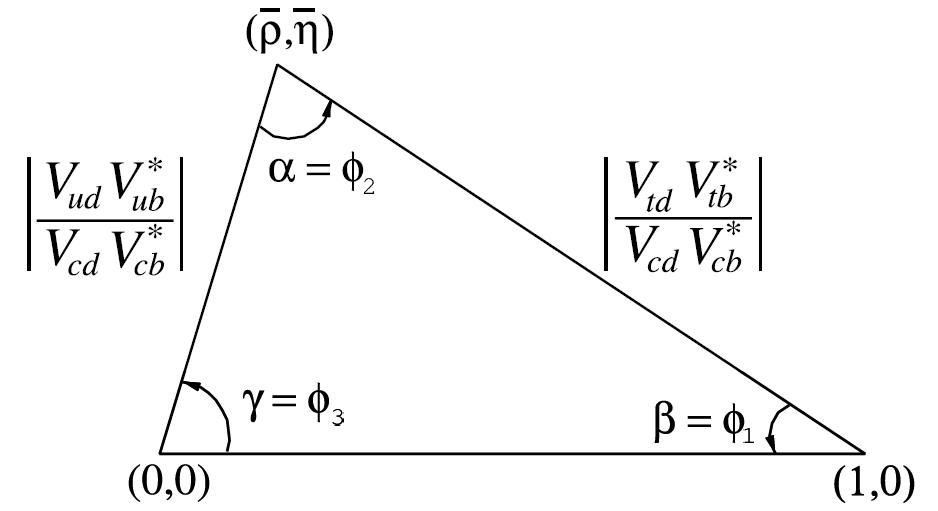
\includegraphics[width=0.5\textwidth]{dreieck}
\caption{Unitaritätsdreieck, entnommen von \cite{dreieck}}
\label{fig:unitarity}
\end{figure}

Das Standardmodell stellt für den hier untersuchten Zerfallskanal eine Beziehung zwischen dem Winkel $\beta$ und der komplexen Größe $\lambda_f$ aus Gleichung \ref{eq:lambda} her (\cite{nir}, \cite{noguchi}):
\begin{align}
&\lambda_f = \underbrace{\frac{V_{td}V_{tb}^*}{V_{td}^*V_{tb}}}_{\frac{q}{p}} \underbrace{\frac{V_{cd}^*V_{cb}}{V_{cd}V_{cb}^*}}_{\frac{\overline{A_f}}{A_f}} = \e^{2\im\beta} \\
\Longrightarrow &\SJPsi = \mathrm{Im}(\lambda_f) = \sin(2\beta).
\end{align}
 
Durch Messung der Amplitude der \CP-Asymmetrie kann man direkte Rückschlüsse auf den CKM-Winkel $\beta$ ziehen, der wesentlicher Bestandteil des Standardmodells ist. \cite{nir}